\section{Background}
\label{background}

Figure \ref{fig:hsa} shows the evolution of the microprocessors.
\begin{figure}[t]
  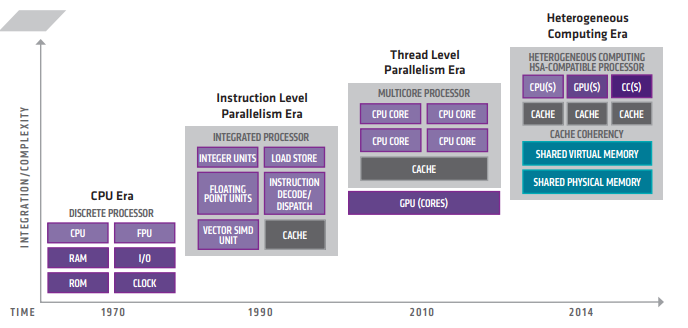
\includegraphics[width=\linewidth]{hsa}
  \caption{Evolution of Microprocessors}
  \label{fig:hsa}
\end{figure}

\subsection{The CPU era} The first processors operated stand-alone, executing
less than a single instruction per clock cycle. Moore's law was driving force
for the evolution at this time. Better performances were gained by increasing
the clock-speed of the processor. Addition of more complex instructions and
also integration of an FPU and math unit in the processor marked significant
development.

\subsection{The Instruction Level Parallelism (ILP) era} Execution of
instructions in parallel that did not have direct data dependencies to each
other was used to improve performance. The development of complex
micro-architectures with parallel units exploiting this instruction level
parallelism (ILP) was the research direction during this phase. This phase saw
the introduction of out-of-order execution and pipelining in the
micro-architectures to increase the instruction per cycle (IPC) count. Addition
of single-instruction-multiple-data (SIMD) also significantly improved the
throughput.

\subsection{Thread Level Parallelism era} Around 2005 the processors hit the
frequency barrier, i.e performance benefits could be achieved by increasing the
frequency, increasing frequency increased the heat dissipated in the chip which
could be fatal to the chip. The research direction during this phase was
breaking down the application in independent threads that could work together
in parallel. Due to Moore's law the increase in the number of transistors was
used to include more processing cores on the same die. This marked the era of
multi-core CPU's. In order to maintain consistent operating results the
processors deployed were expected to be identical to each other forming a
symmetric-multi-processor (SMP) system. This new generation of processors was
classified by CPU core count

\subsection{Discrete GPU era} The increase in graphic-intensive applications
around 2000 led to the addition of a specialized graphics processing unit to
the existing architecture. The combination of discrete GPUs into systems with
CPUs significantly improved performance. Applications isolated portions and
offloaded them to both the compute units and gained significant throughput.
This also led to the development of the CUDA and OpenCL programming models.

\subsection{Heterogeneous Computing era} The integration of CPU and GPU in a
single chip marks this phase. Being on a single chip opened new avenues of
sharing memory across both the compute units. Limitations due to Moore's law
and Dennard Scaling paved the way for this architecture to dominate the
mainstream markets. The transition to heterogeneous computing where various
execution units are more thightly integrated and share system resources, is
directly proportional to the market pressure and need for higher performance,
power efficiency and cost for the end user. This can be clearly seen in the
systems we interact with nowadays. From embdeded devices to super computers all
implement heterogenous architecture. Most of the research today is directed
towards automatic partitioning of work for the compute devices.

